\documentclass[aspectratio=169]{beamer}

\usetheme{Warsaw}
\usecolortheme{default}

\usepackage[T1]{fontenc}
\usepackage[utf8]{inputenc}
\usepackage{lmodern}
\usepackage{graphicx}
\usepackage{booktabs}
\usepackage{amsmath}
\usepackage{amssymb}
\usepackage{xcolor}

\graphicspath{{../outputs/plots/}}

\definecolor{PUT-blue}{RGB}{0,84,147}
\definecolor{PUT-dark}{RGB}{0,45,85}
\definecolor{highlight}{RGB}{230,126,34}

\setbeamercolor{palette primary}{bg=PUT-blue,fg=white}
\setbeamercolor{palette secondary}{bg=PUT-dark,fg=white}
\setbeamercolor{palette tertiary}{bg=PUT-blue,fg=white}
\setbeamercolor{structure}{fg=PUT-blue}
\setbeamertemplate{headline}{}

\setbeamerfont{title}{size=\LARGE}
\setbeamerfont{frametitle}{size=\Large}
\setbeamerfont{normal text}{size=\normalsize}
\setbeamerfont{itemize/enumerate body}{size=\normalsize}

\title{Cluster Validity Study}
\subtitle{A Data-Driven Comparative Analysis}
\author{Pawe\l{} Florek}
\institute{Warsaw University of Technology}
\date{\today}

\begin{document}

\begin{frame}[plain]
    \titlepage
\end{frame}

\begin{frame}{Analytical Purpose}
    \begin{itemize}
        \item Compare average performance across method families.
        \item Examine consistency of algorithm rankings across different metrics.
        \item Analyze the correlation structure of metrics and its implications for evaluation.
        \item Investigate the sensitivity of different algorithms to their hyperparameters and their performance across different dataset batteries.
    \end{itemize}
\end{frame}

\section{Overall results}
\begin{frame}{External Metrics Distribution}
    \centering
    \includegraphics[width=0.70\textwidth]{external_metrics_violin.png}
    \\[0.1em]
    {\small Separation between robust methods and highly parameter-sensitive methods.}
\end{frame}

\section{External vs Internal Metrics}

\begin{frame}{Metric Correlation Structure}
    \begin{columns}
        \column{0.75\textwidth}
        \centering
        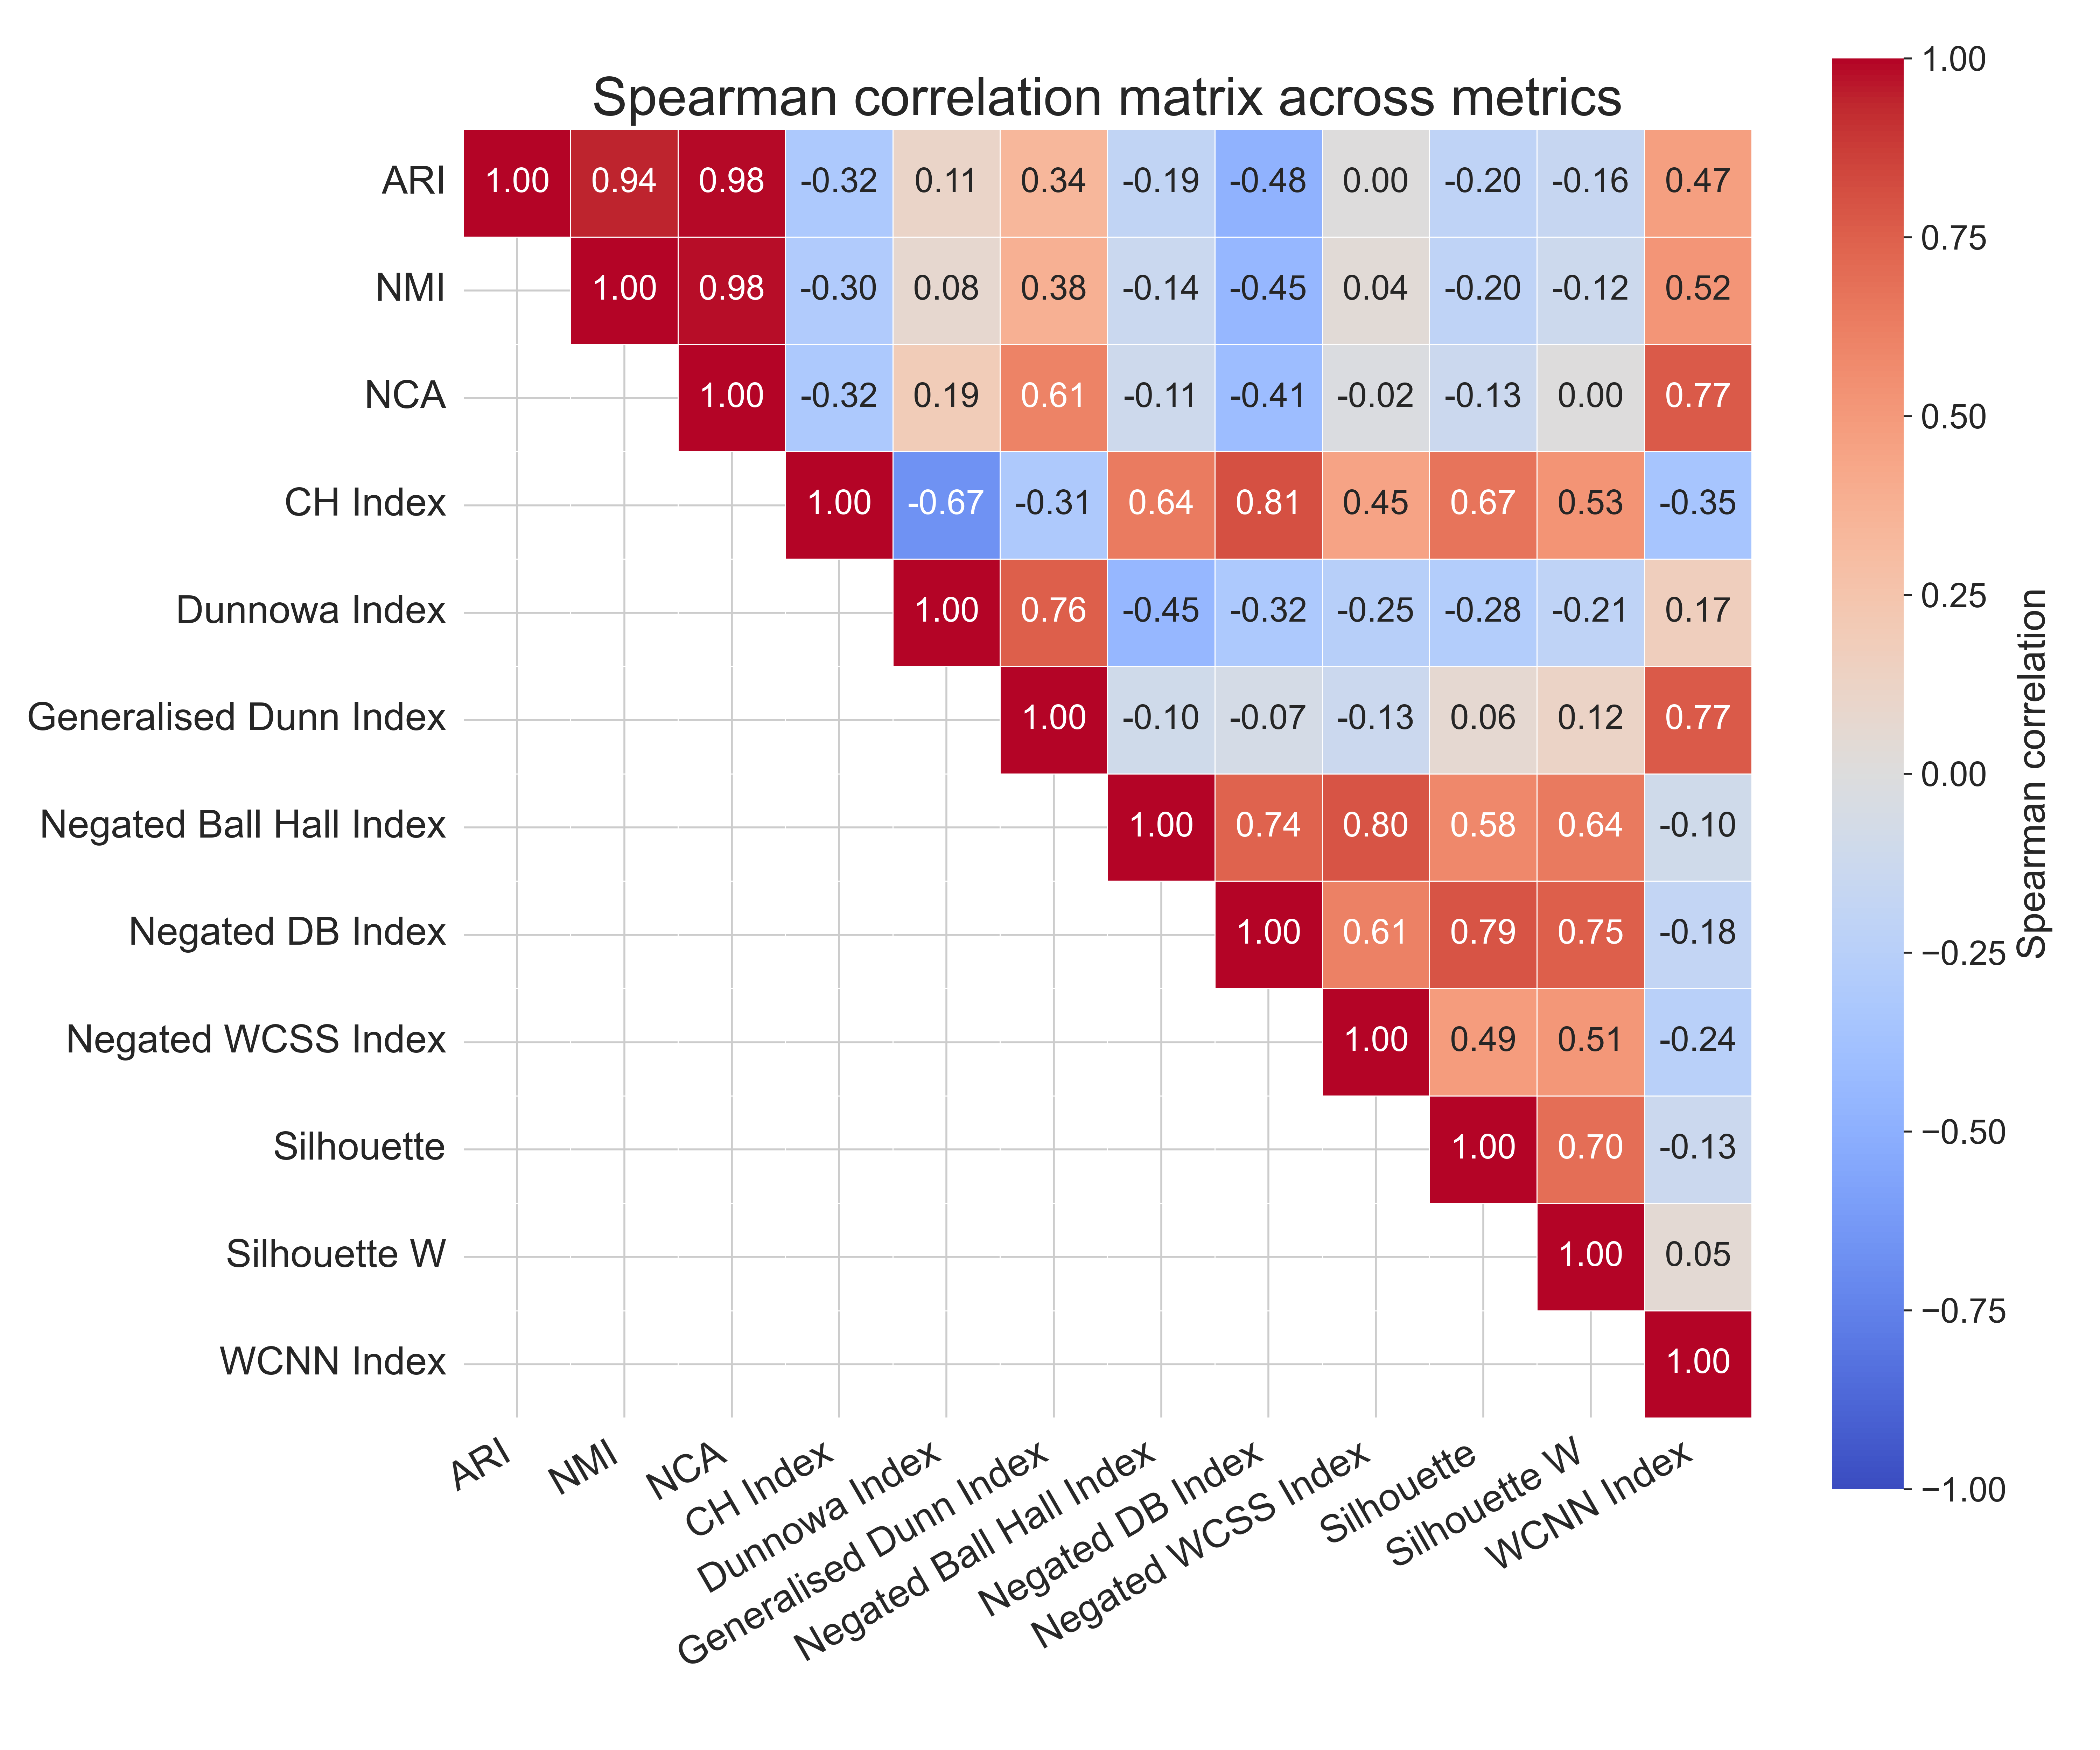
\includegraphics[width=0.95\textwidth]{metric_spearman_correlation.png}

        \column{0.25\textwidth}
        {\small Strong agreement inside external metrics, weaker agreement between external and internal metrics.}
    \end{columns}
\end{frame}

\begin{frame}{Ranking Stability Across Metrics}
    \centering
    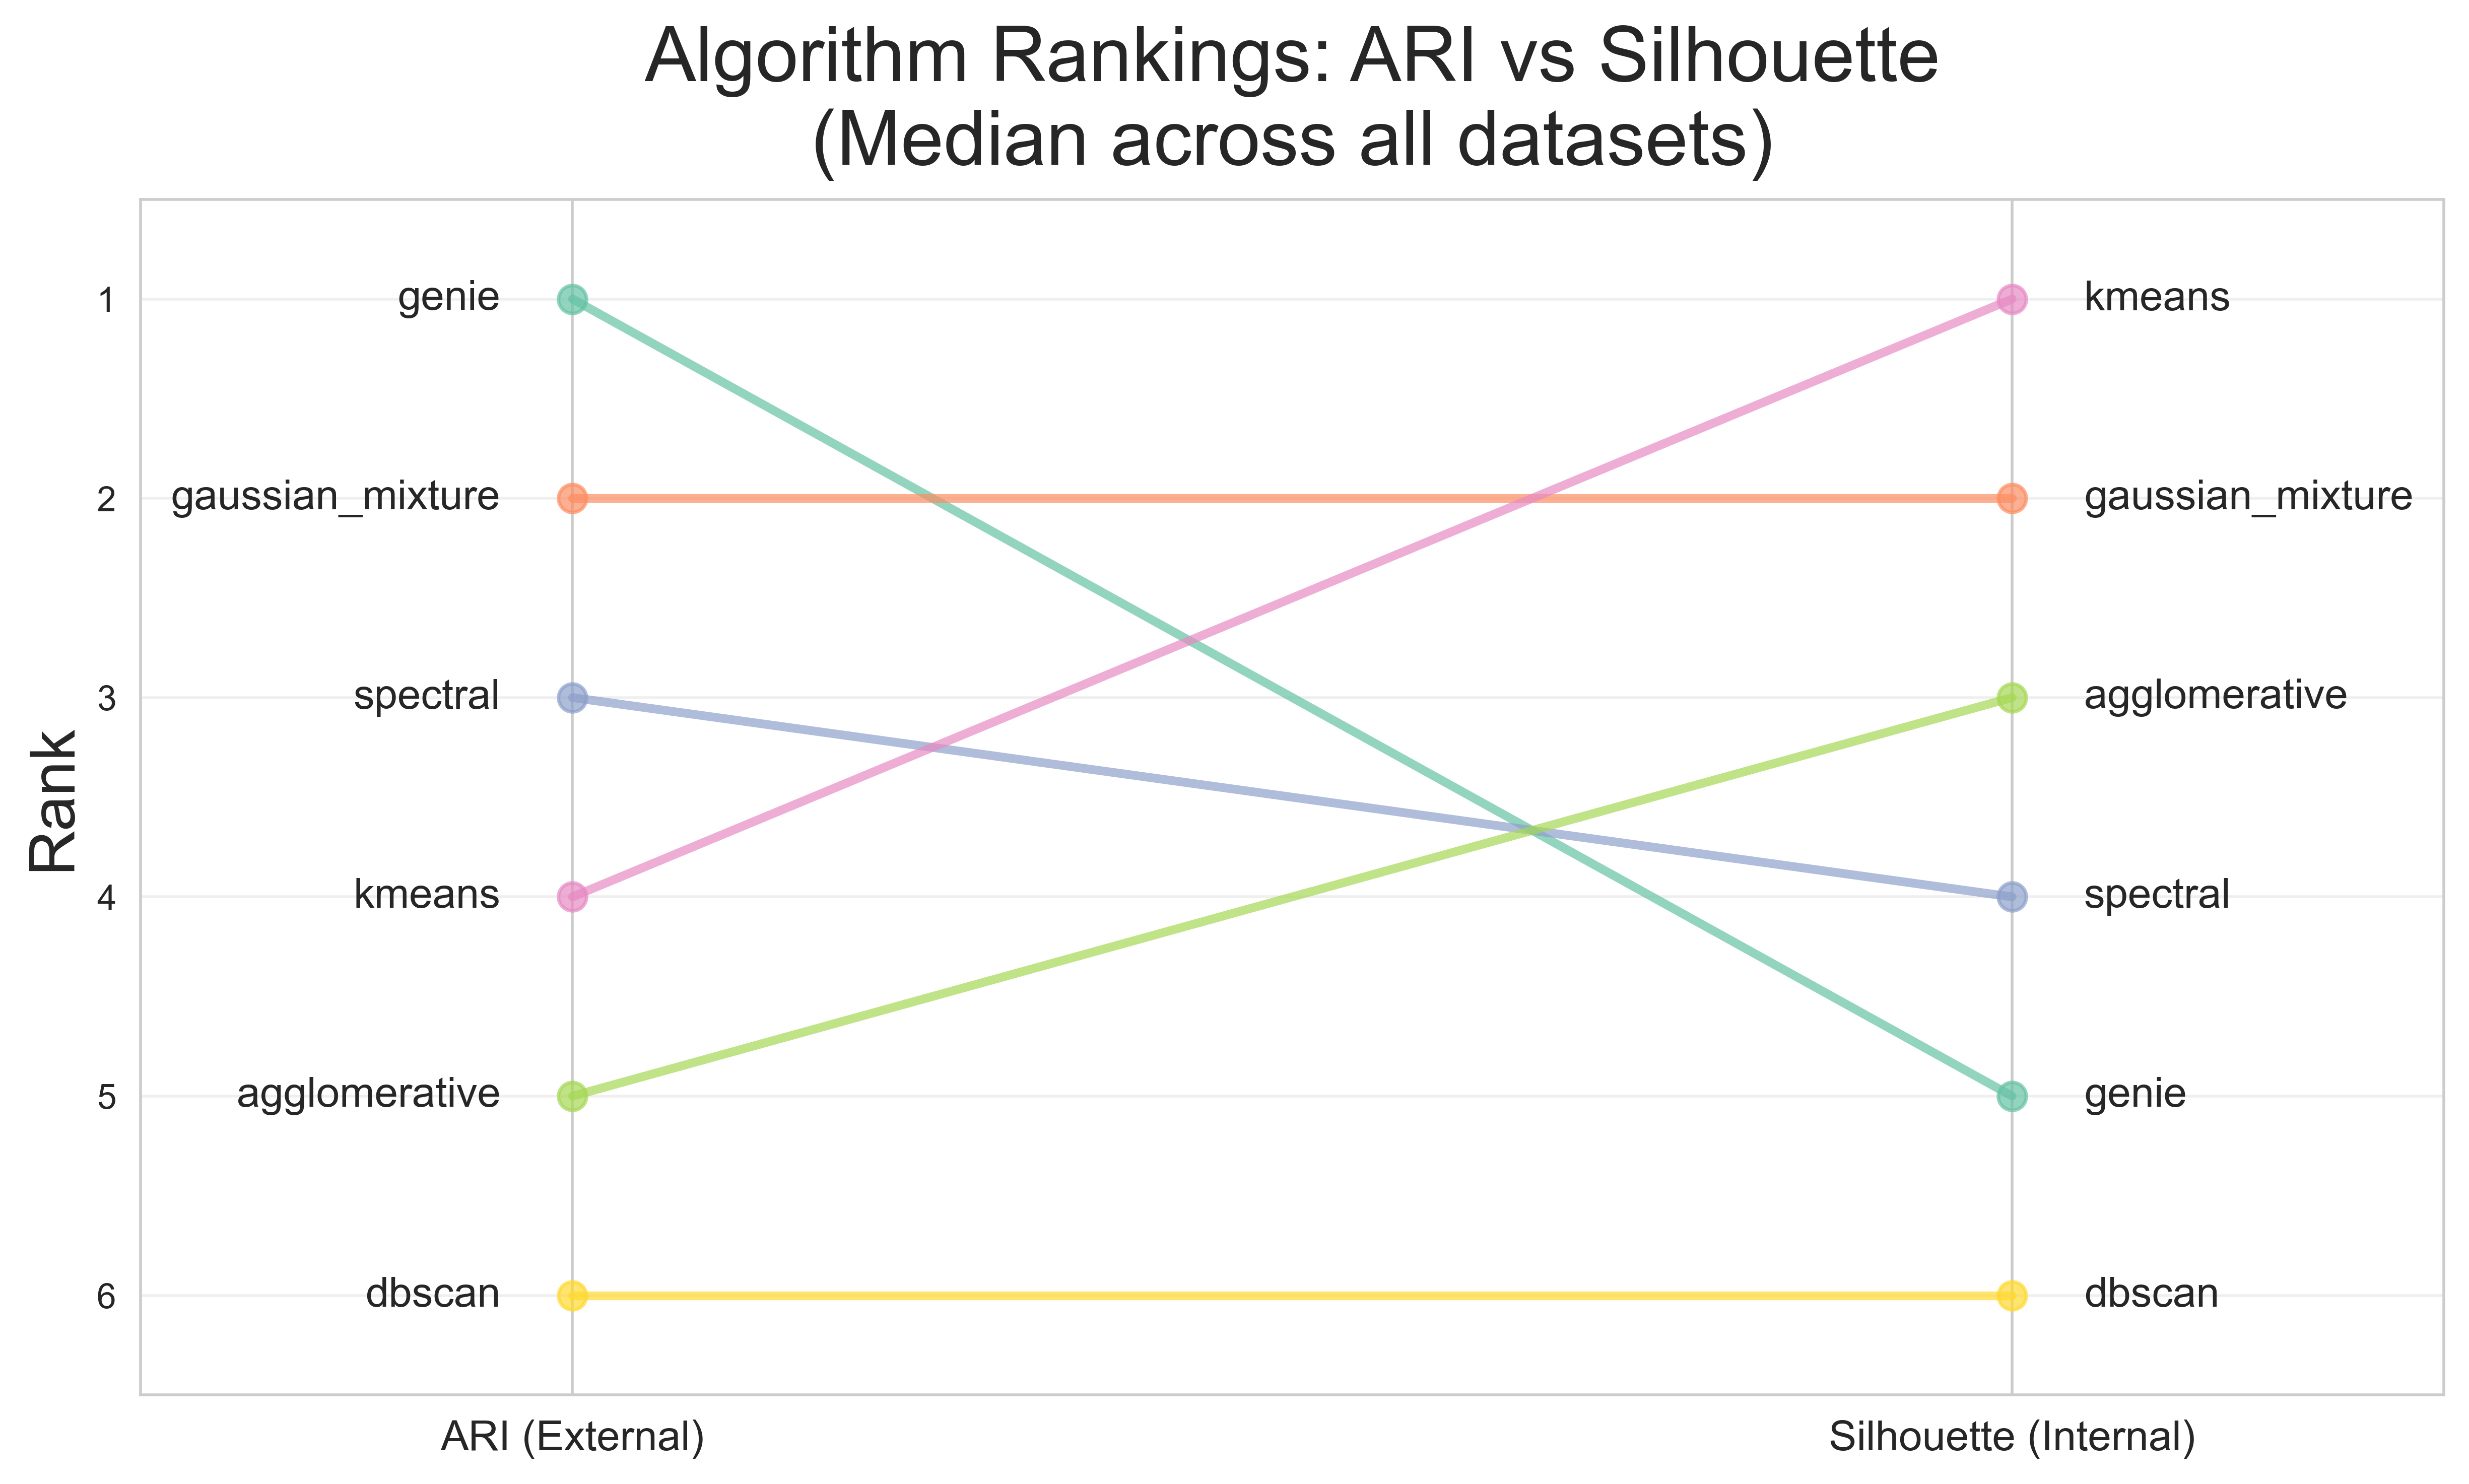
\includegraphics[width=0.80\textwidth]{algorithm_rankings_slopegraph.png}
    \\[0.1em]
    {\small Rankings shift with the metric.}
\end{frame}

\begin{frame}{Reading the Consistency Pattern}
    \begin{itemize}
        \item Internal criteria reflect different properties of partitions.
        \item Rankings can change depending on the metric family.
        \item A mixed evaluation protocol might give a more reliable picture.
    \end{itemize}
\end{frame}

\begin{frame}{Low correlation: Silhouette vs ARI}
    \centering
    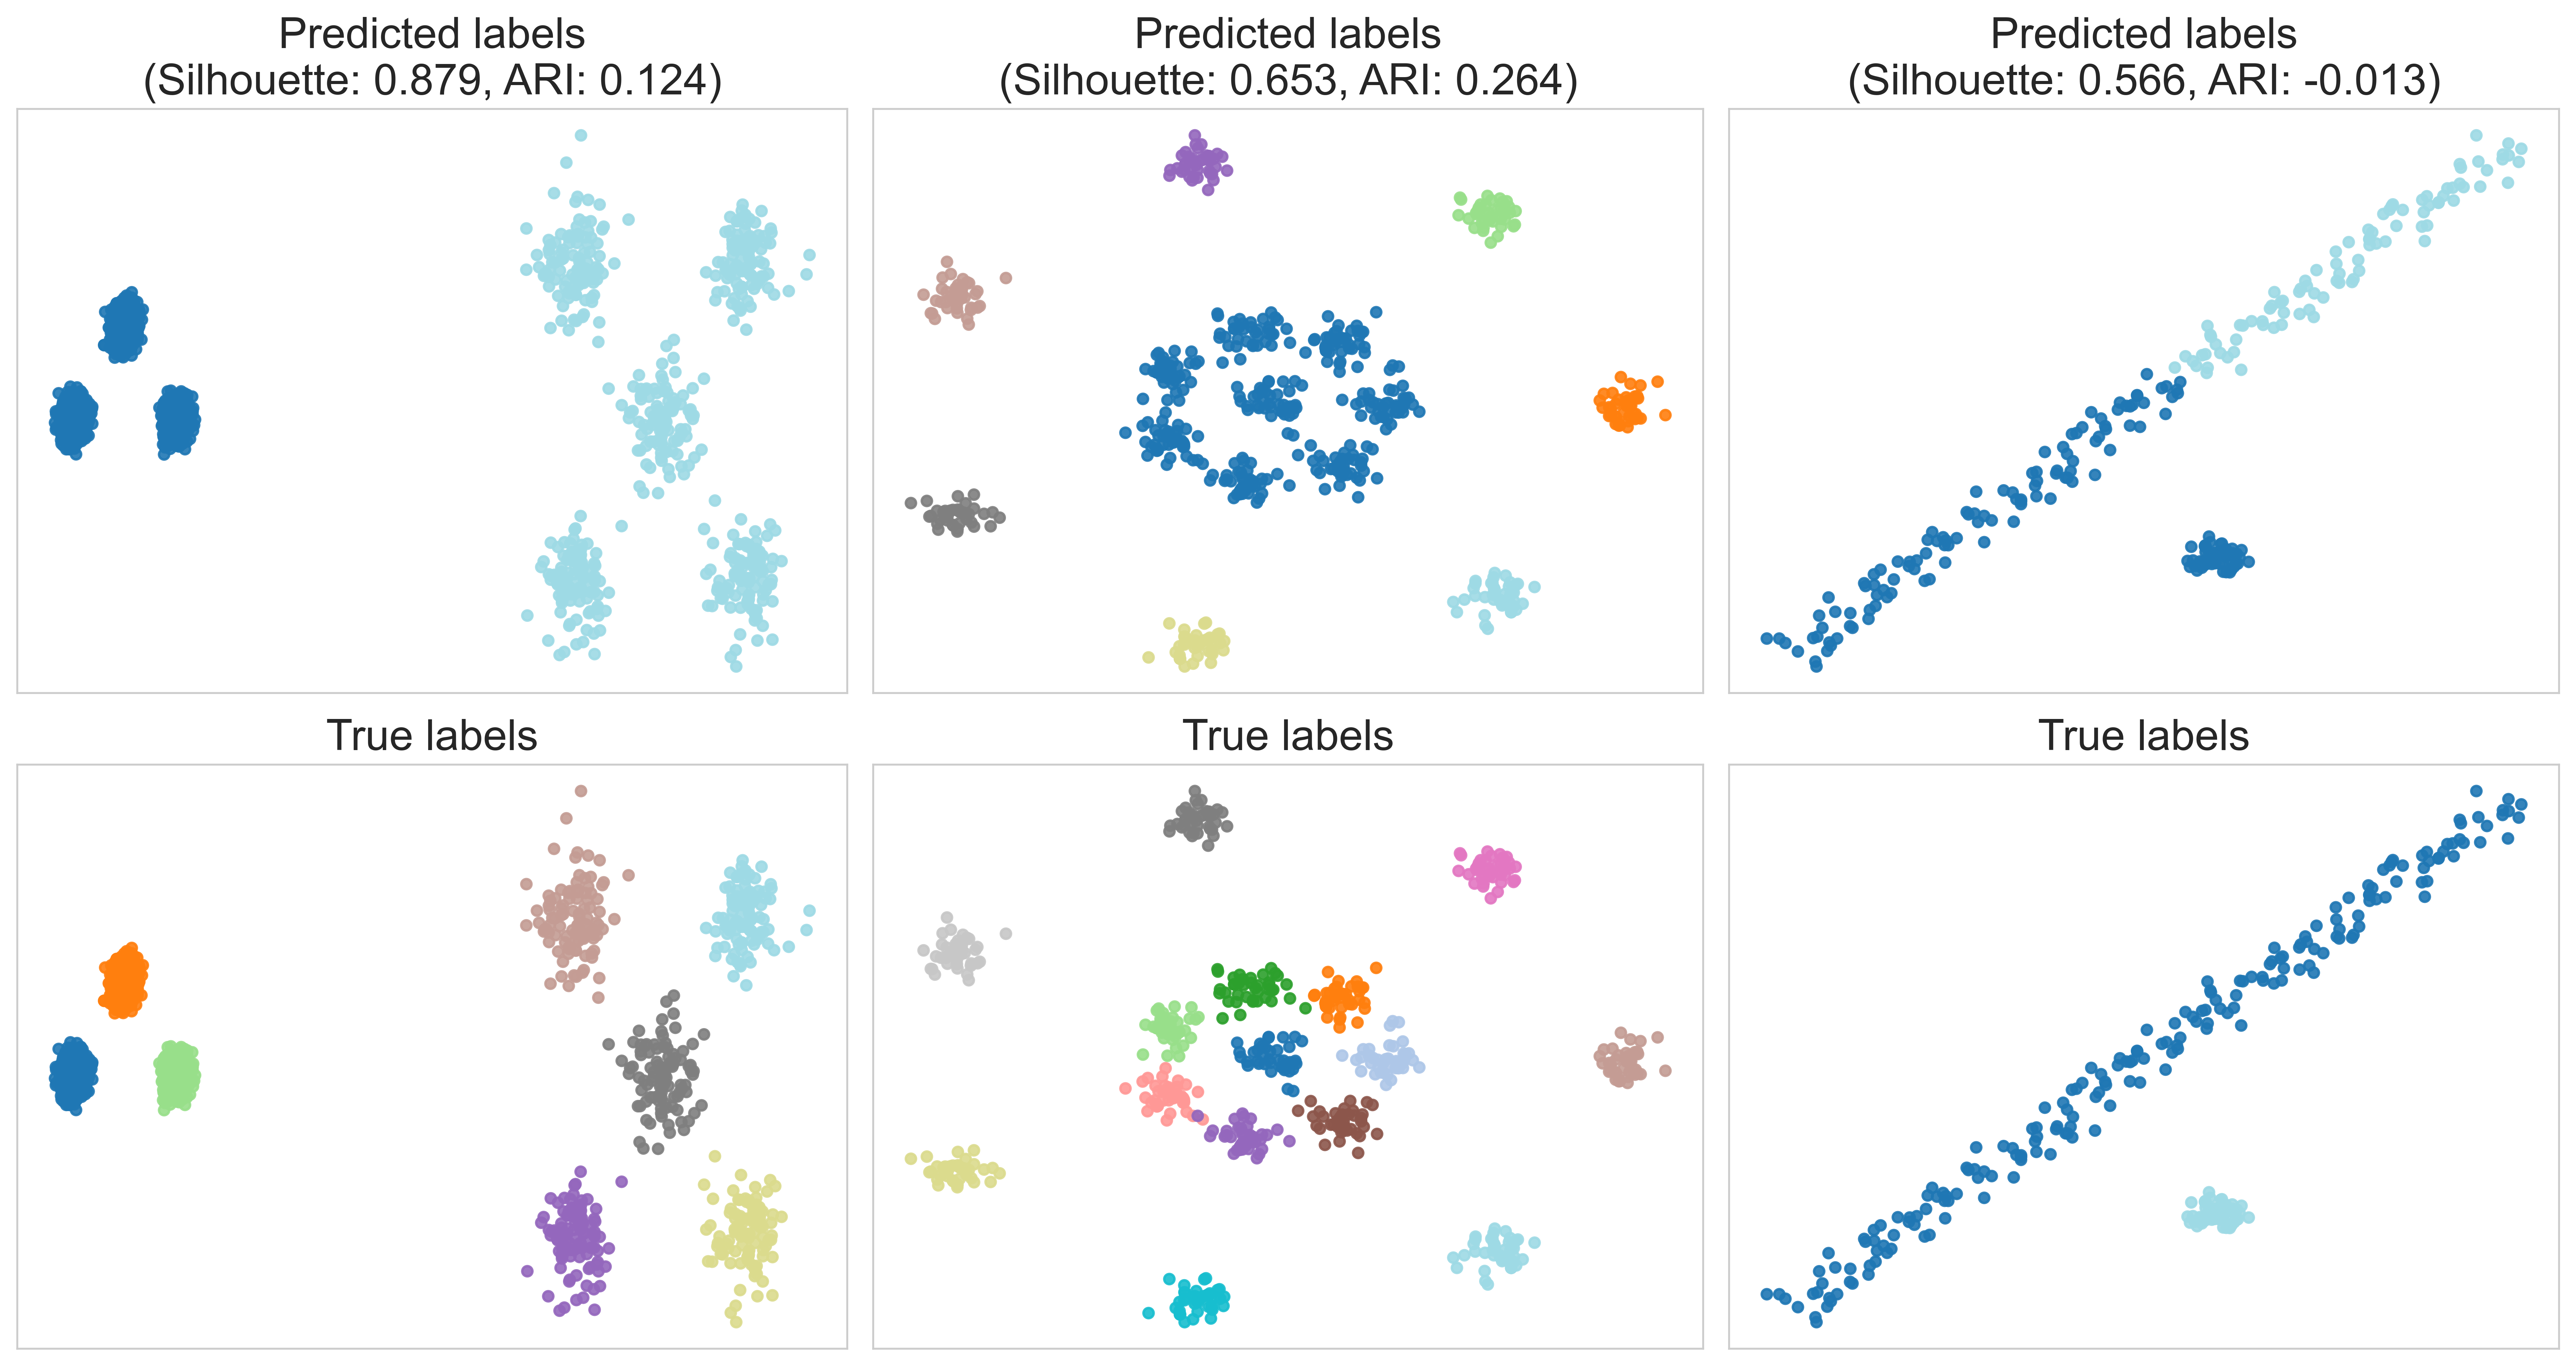
\includegraphics[width=0.90\textwidth]{high_silhouette_low_ari_examples.png}
    \\[0.1em]
    {\small High separation/compactness can coexist with weak agreement to ground truth labels\\
    (ARI $<$ 0.25 quantile, Silhouette $>$ 0.75 quantile).}
\end{frame}

\begin{frame}{Low correlation: Negated WCSS vs ARI}
    \centering
    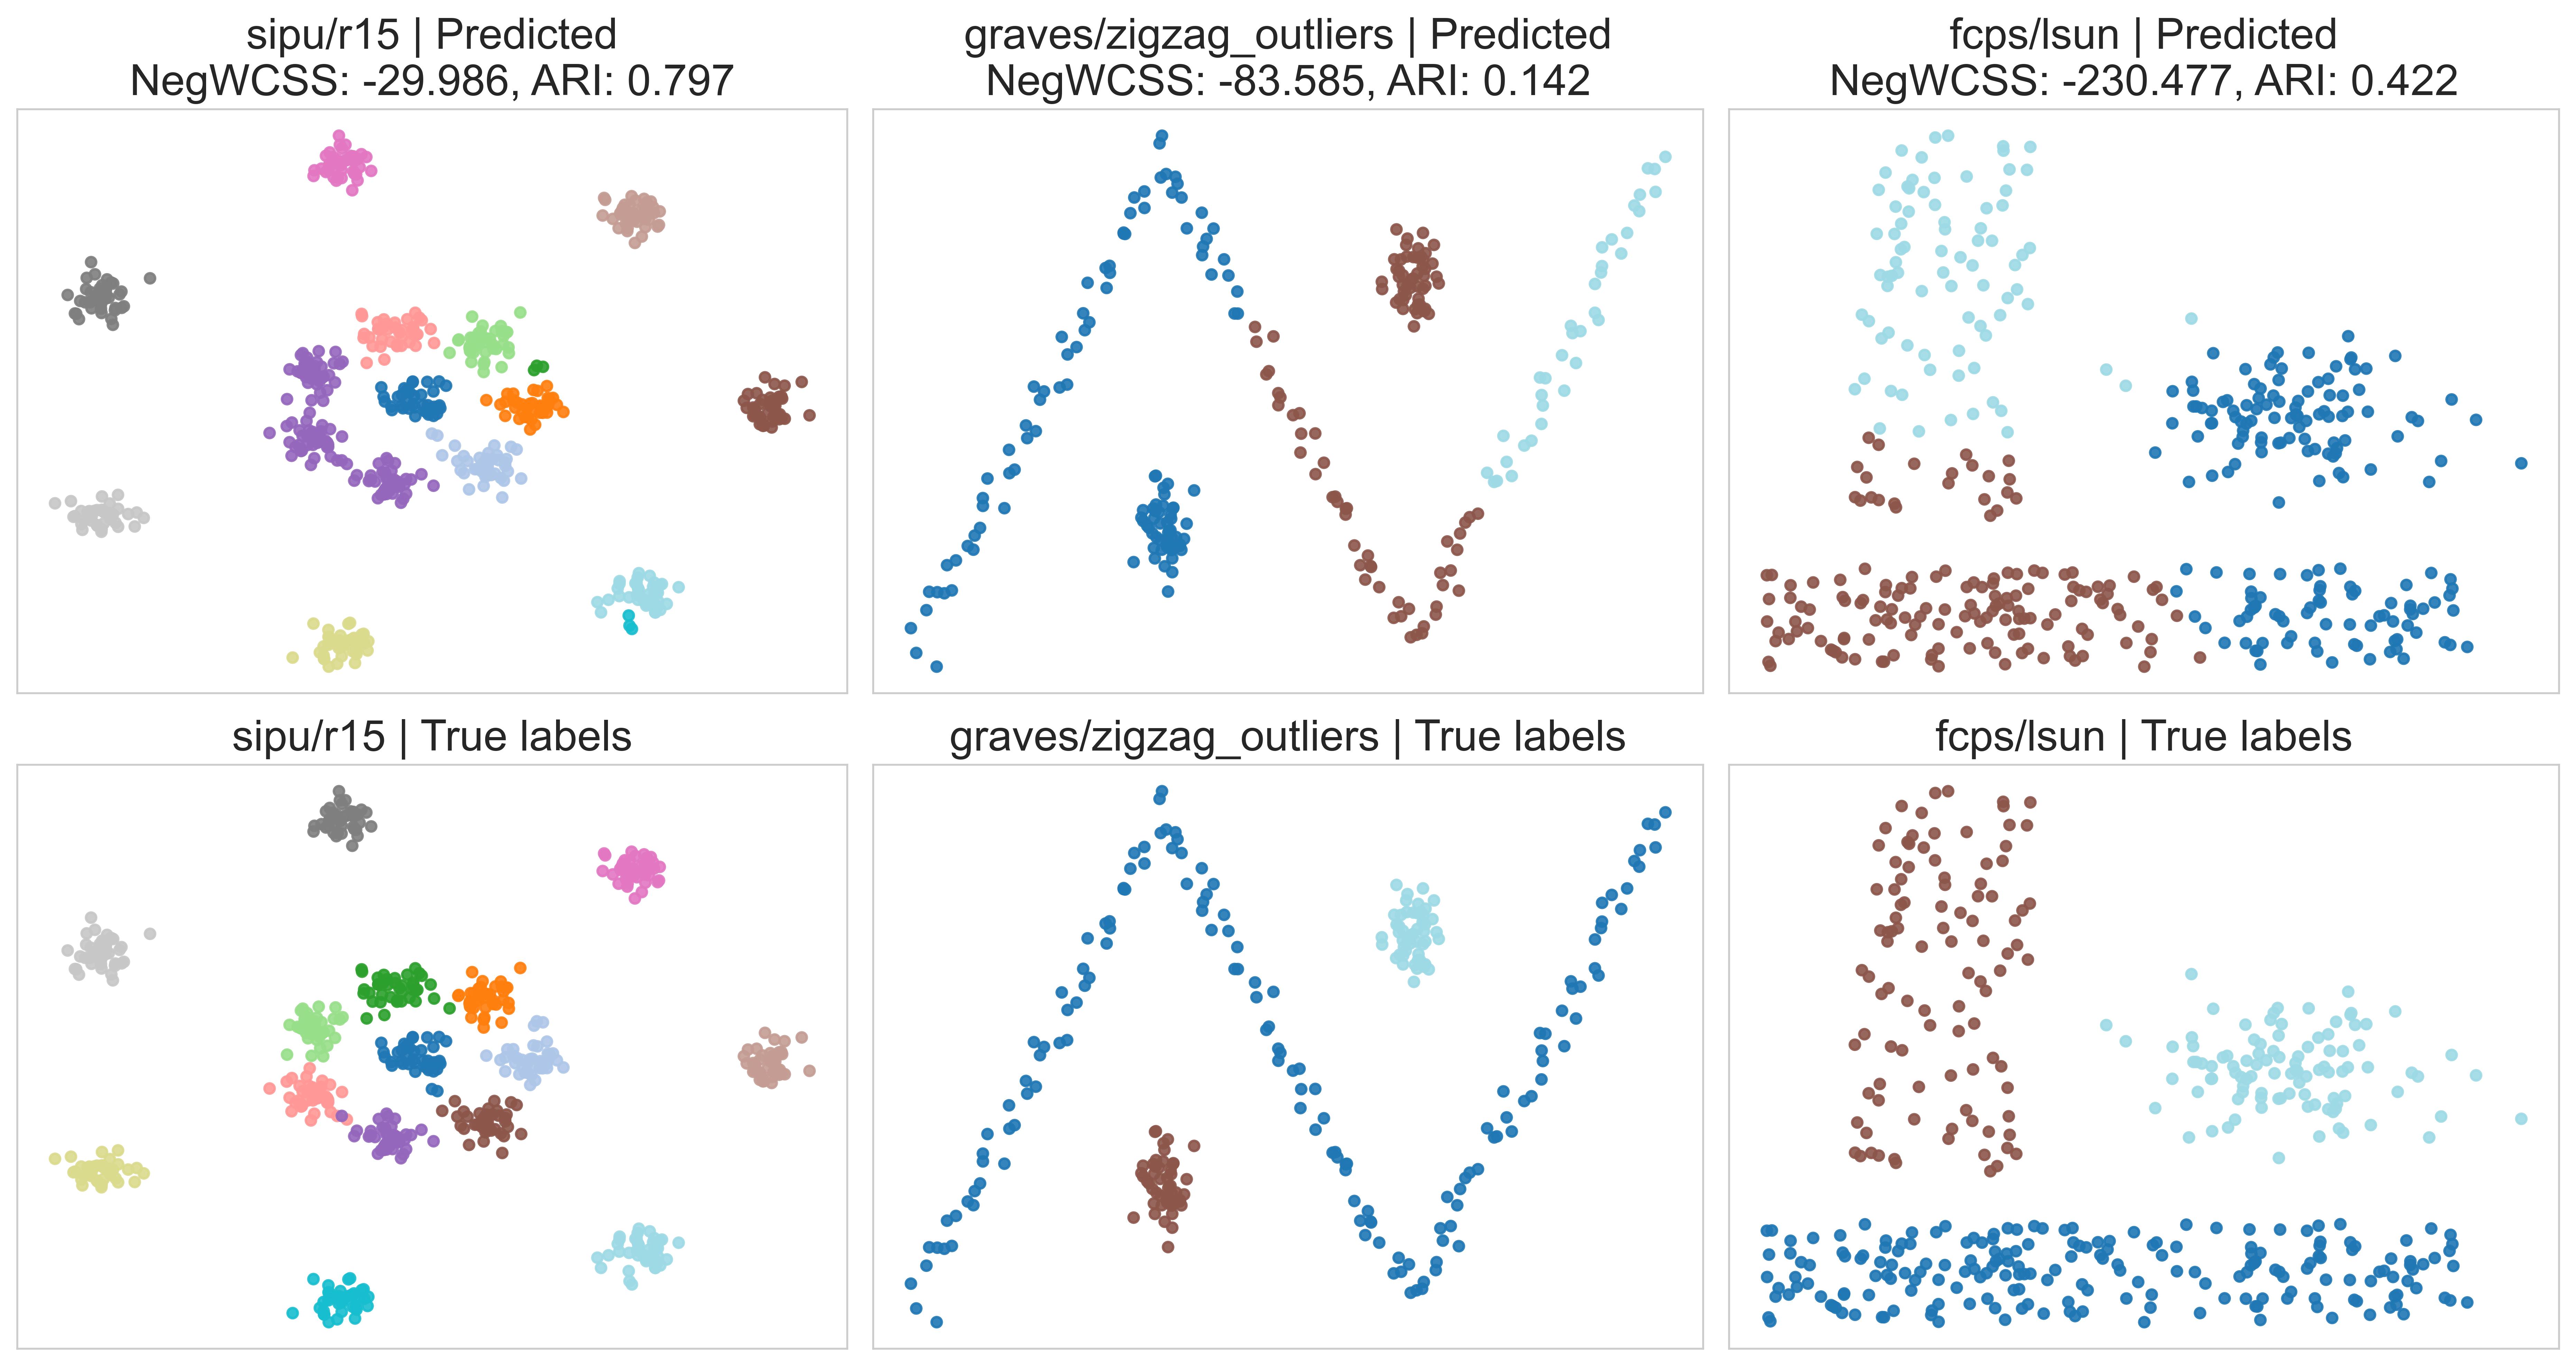
\includegraphics[width=0.90\textwidth]{high_negated_wcss_low_ari_examples.png}
    \\[0.1em]
    {\small Compact partitions are not always semantically meaningful partitions\\
    (ARI $<$ 0.5 quantile, Negated WCSS $>$ 0.7 quantile).}
\end{frame}

\begin{frame}{Implications for Internal Metrics}
    \begin{itemize}
        \item Internal measures remain useful for geometric diagnostics.
        \item As standalone selectors, they may favor misleading solutions.
        \item They work best as complementary evidence.
        \item External references are important whenever available.
    \end{itemize}
\end{frame}

\begin{frame}{DBSCAN Sensitivity hyperparameters}
    \centering
    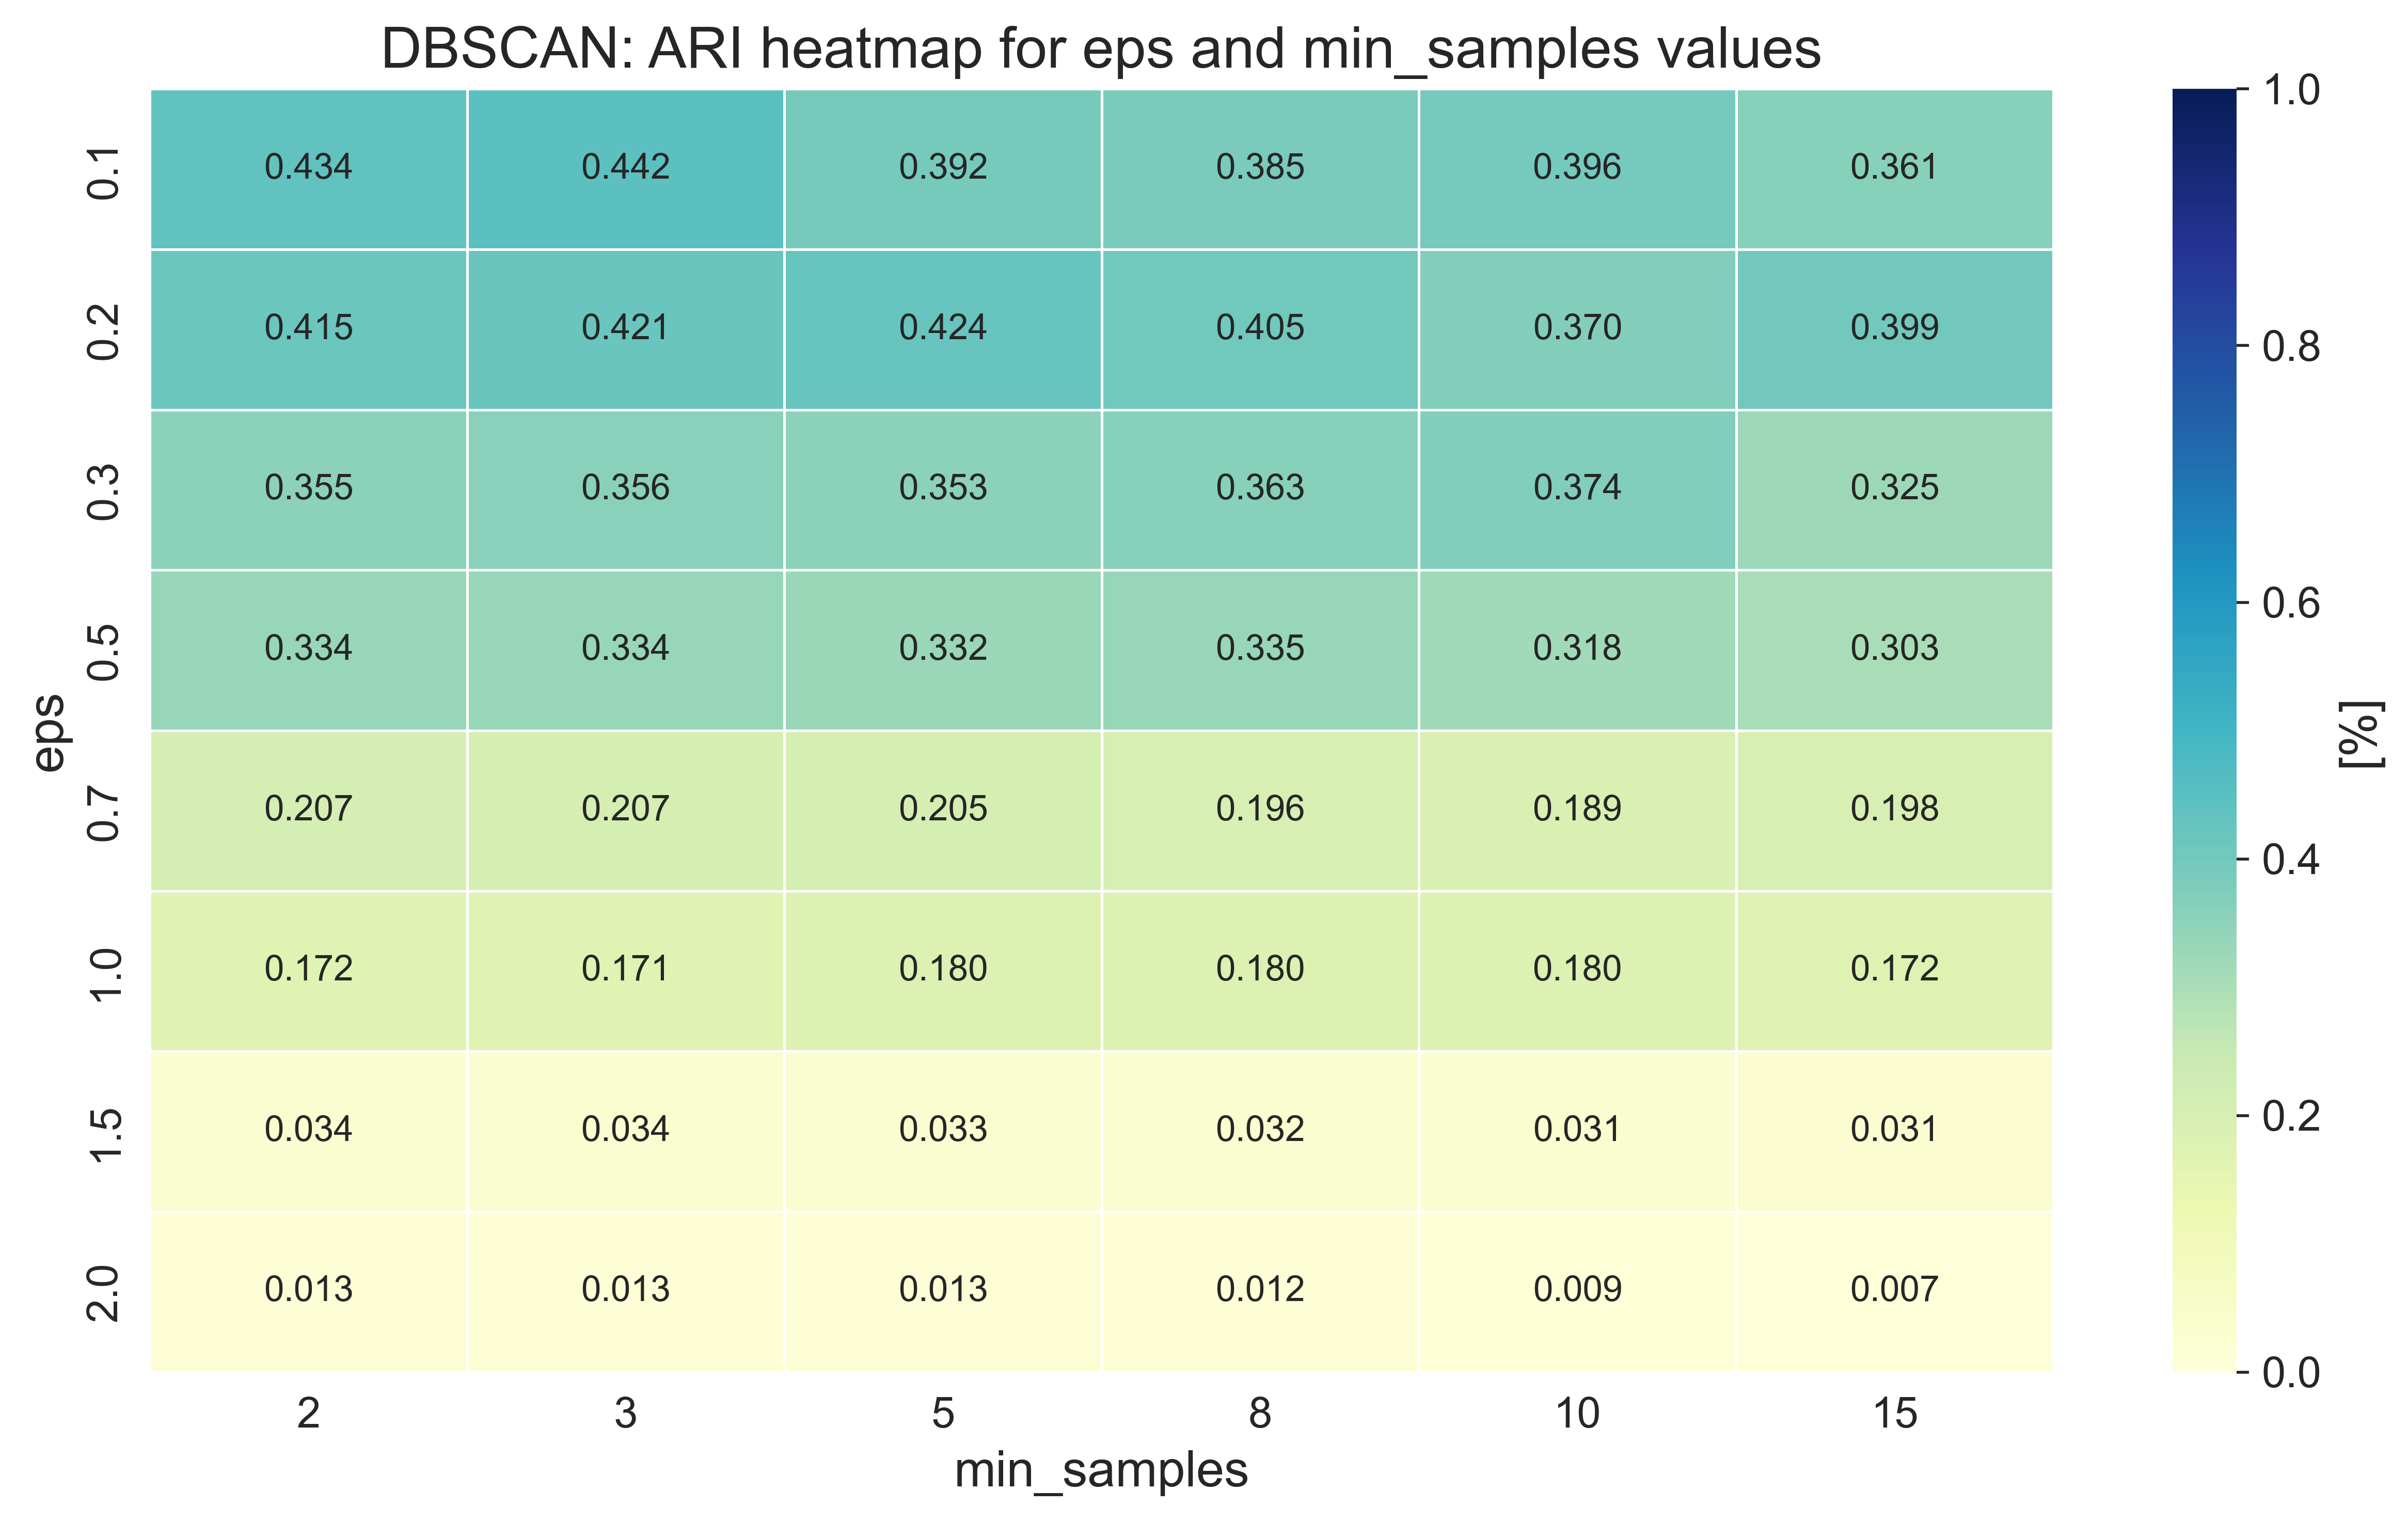
\includegraphics[width=0.85\textwidth]{dbscan_ari_eps_min_samples.png}
\end{frame}

\begin{frame}{DBSCAN results on different batteries}
    \centering
    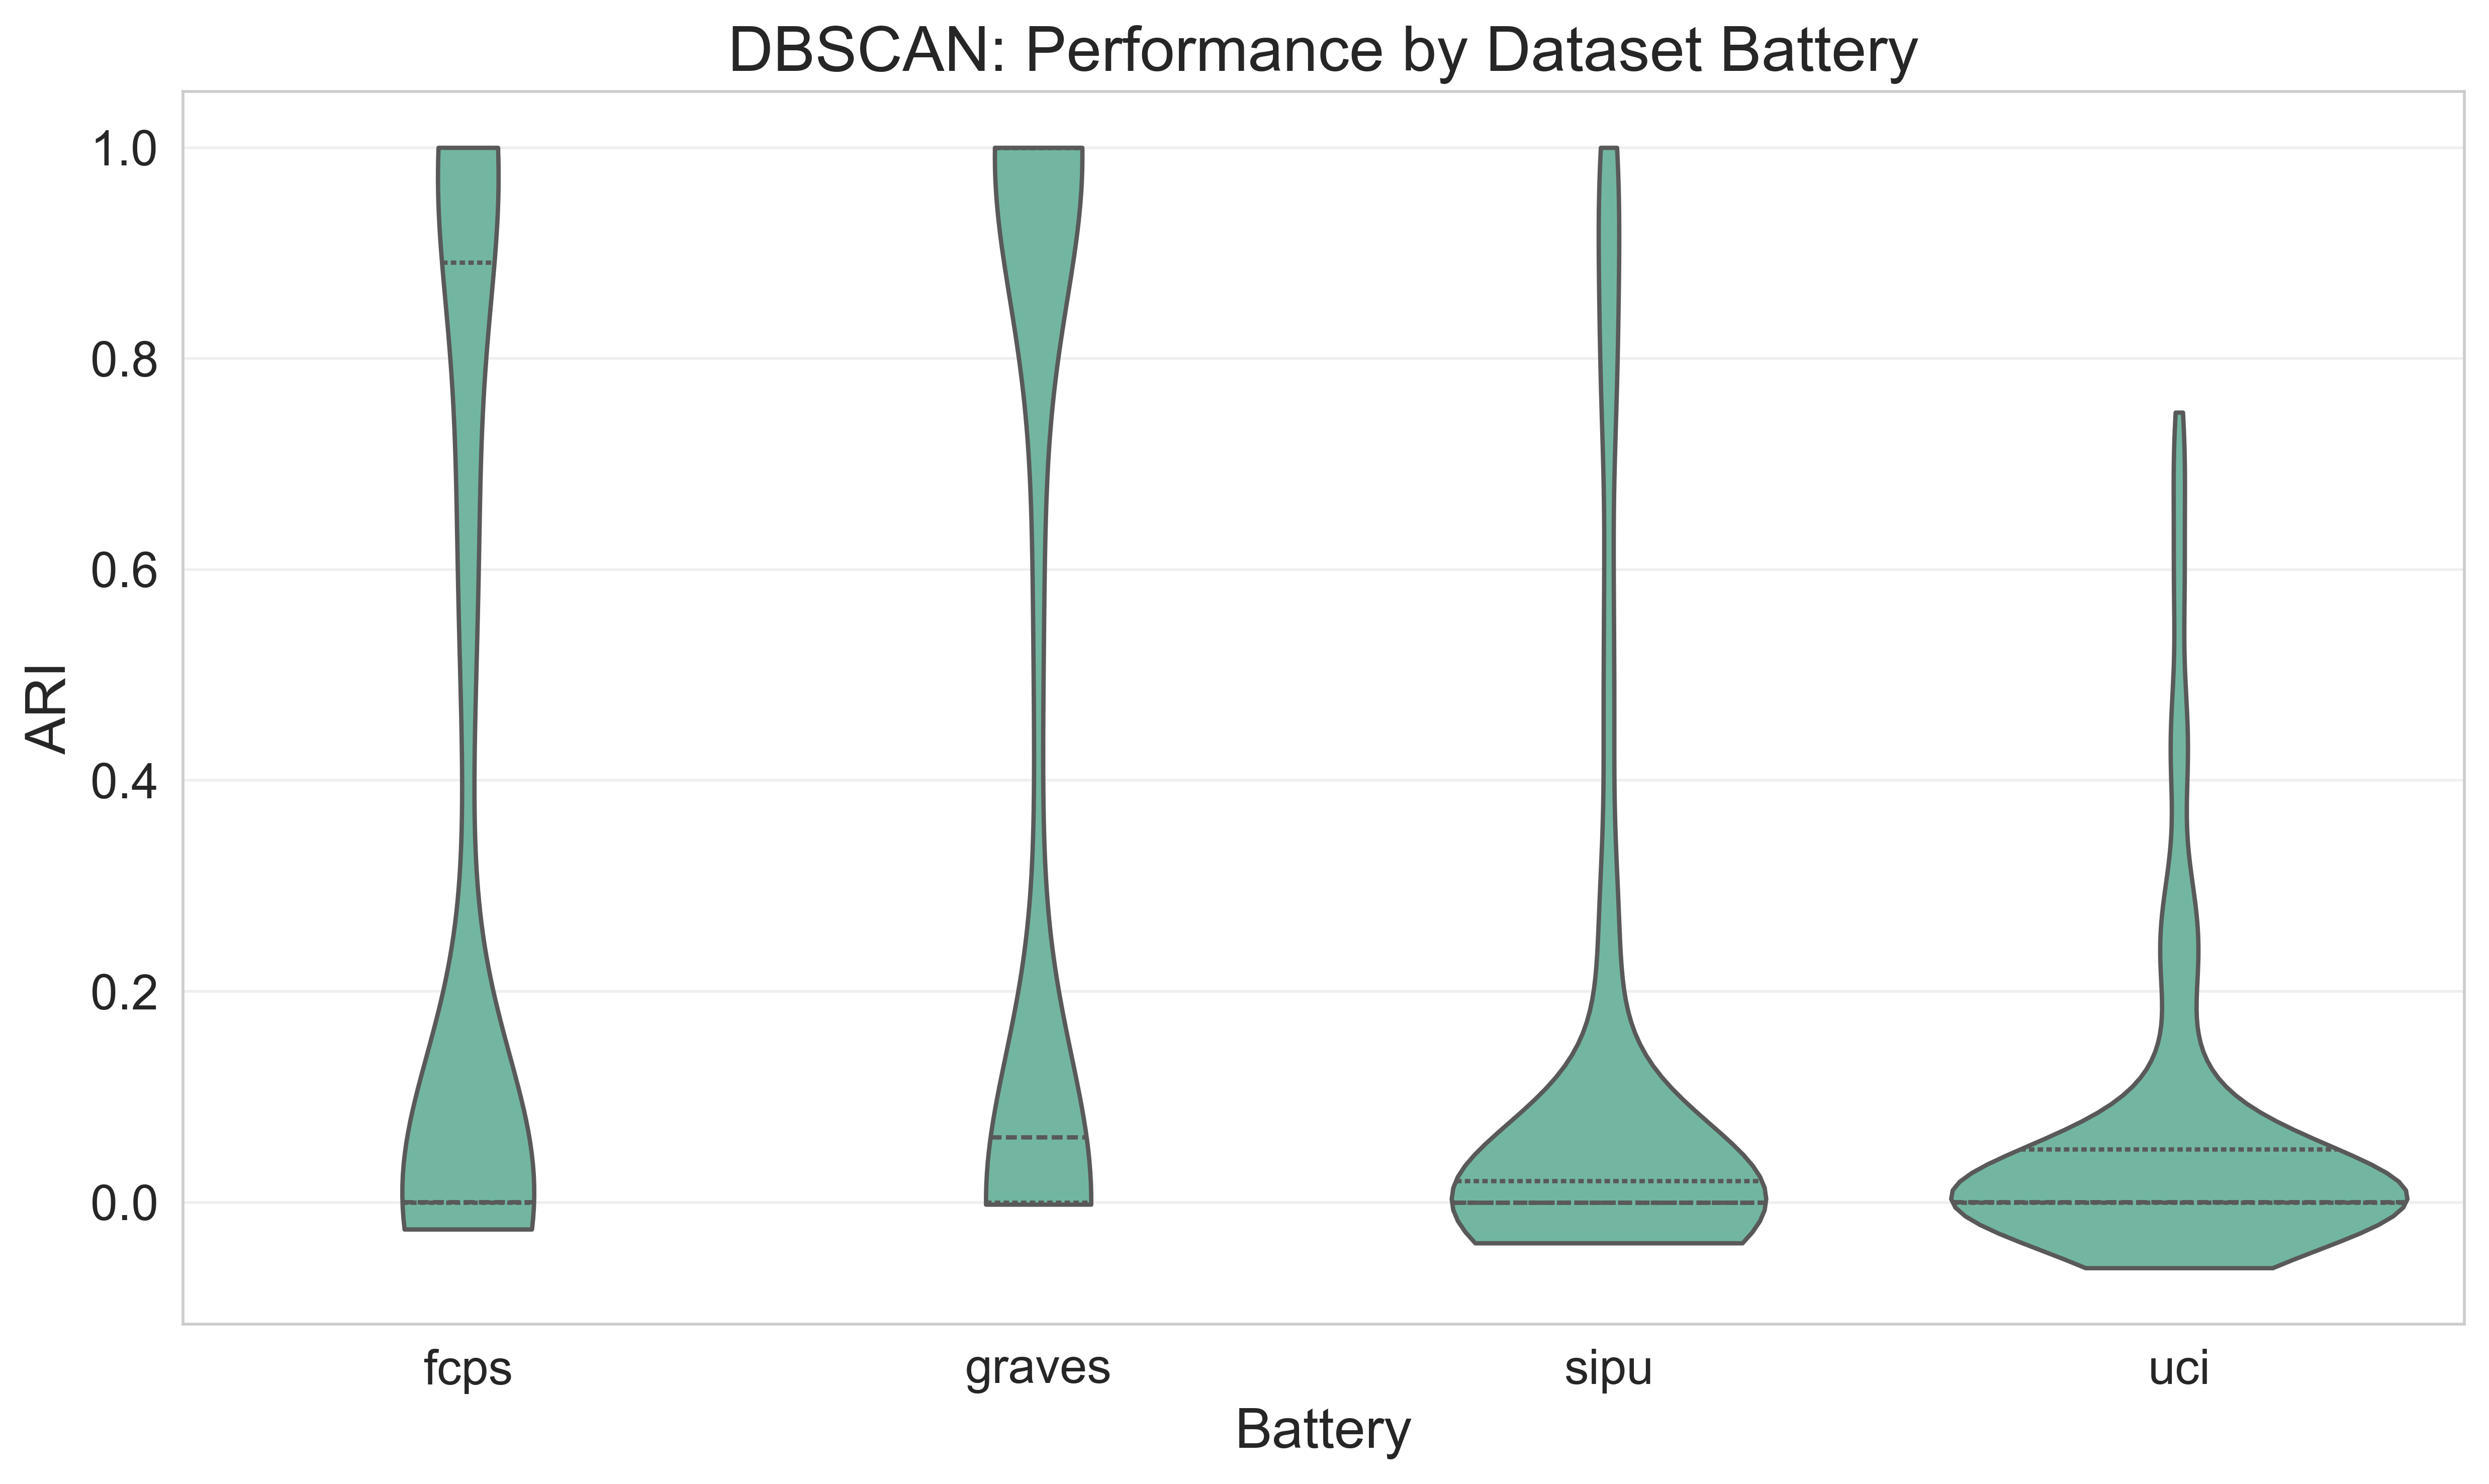
\includegraphics[width=0.85\textwidth]{dbscan_ari_by_battery.png}
    \\[0.1em]
    {\small DBSCAN can excel on some datasets, but fails on others without careful tuning.}

\end{frame}

\begin{frame}{Best DBSCAN Configuration by Battery}
    \centering
    \begin{tabular}{lccc}
        \toprule
        Battery & eps & min\_samples & ARI \\
        \midrule
        fcps   & 0.7 & 2  & 1.000000 \\
        graves & 0.1 & 8  & 1.000000 \\
        sipu   & 0.2 & 15 & 1.000000 \\
        uci    & 0.1 & 5  & 0.748956 \\
        \bottomrule
    \end{tabular}
\end{frame}

\begin{frame}{DBSCAN Noise Profile by Battery}
     \centering
     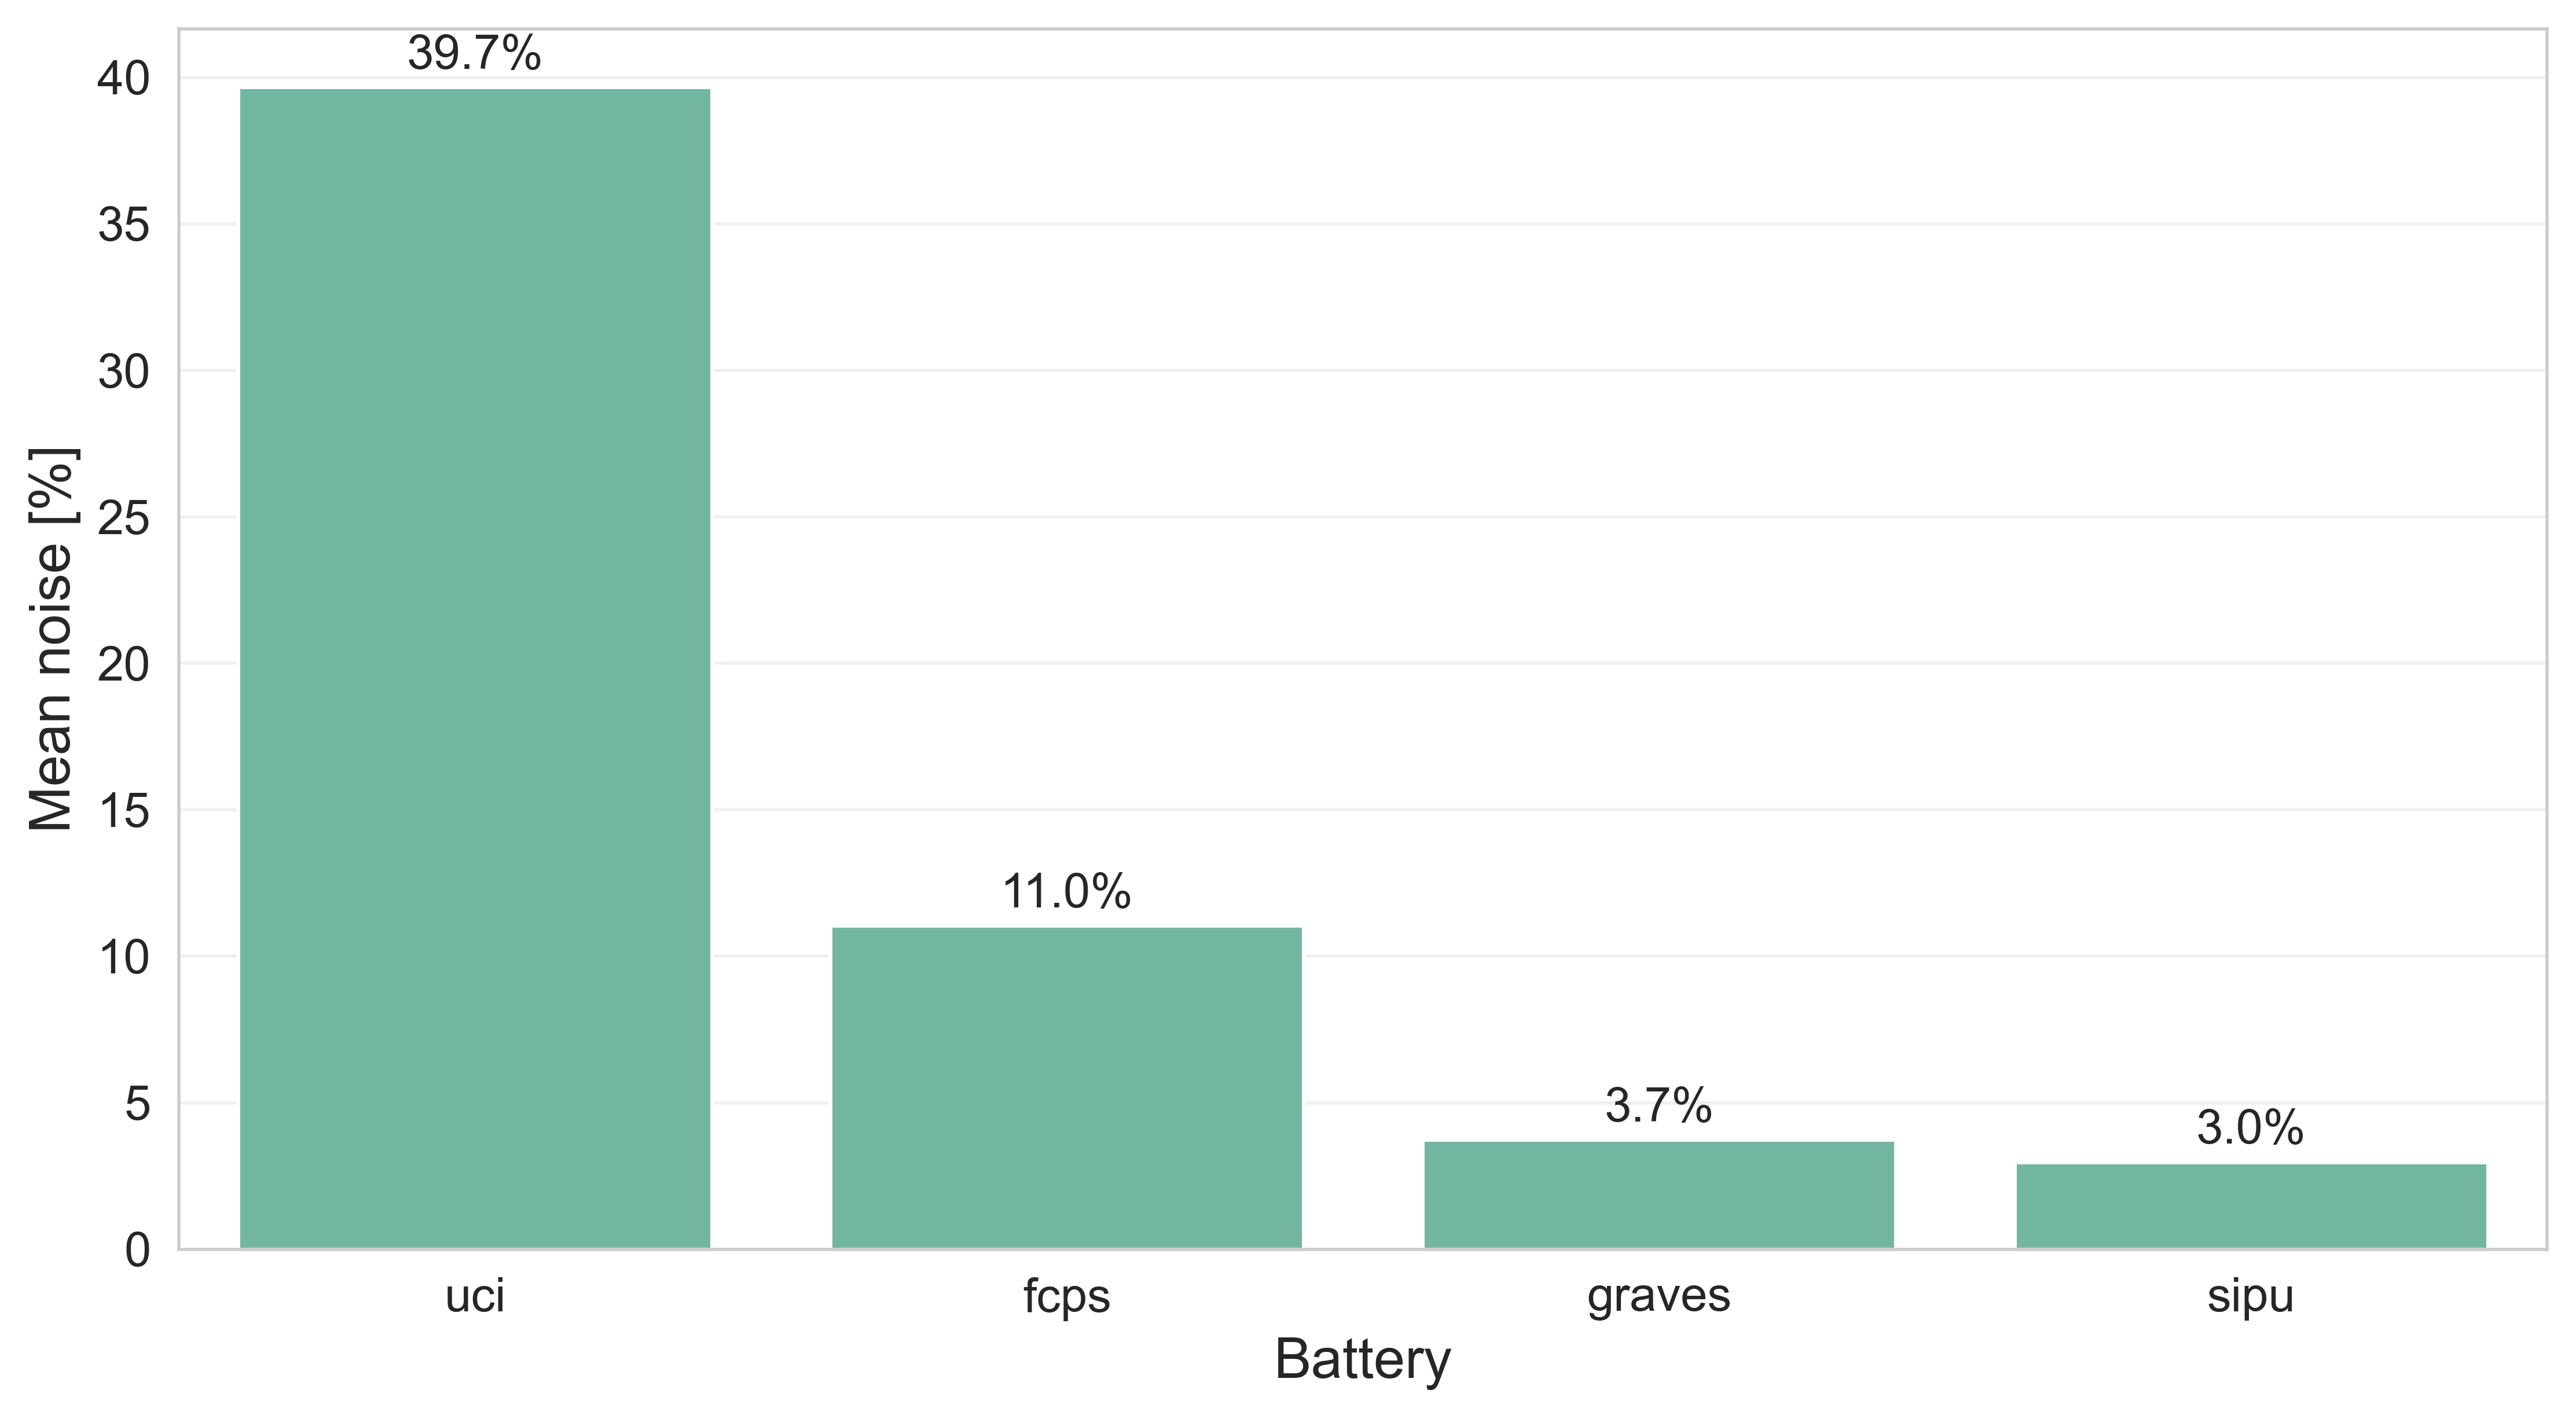
\includegraphics[width=0.65\textwidth]{dbscan_mean_noise_pct_by_battery.png}
     \\[0.1em]
     {\small Mean noise share differs across batteries, indicating density mismatch between one global setting and local data structure.}
\end{frame}

\begin{frame}{Genie Sensitivity to $g$}
    \centering
    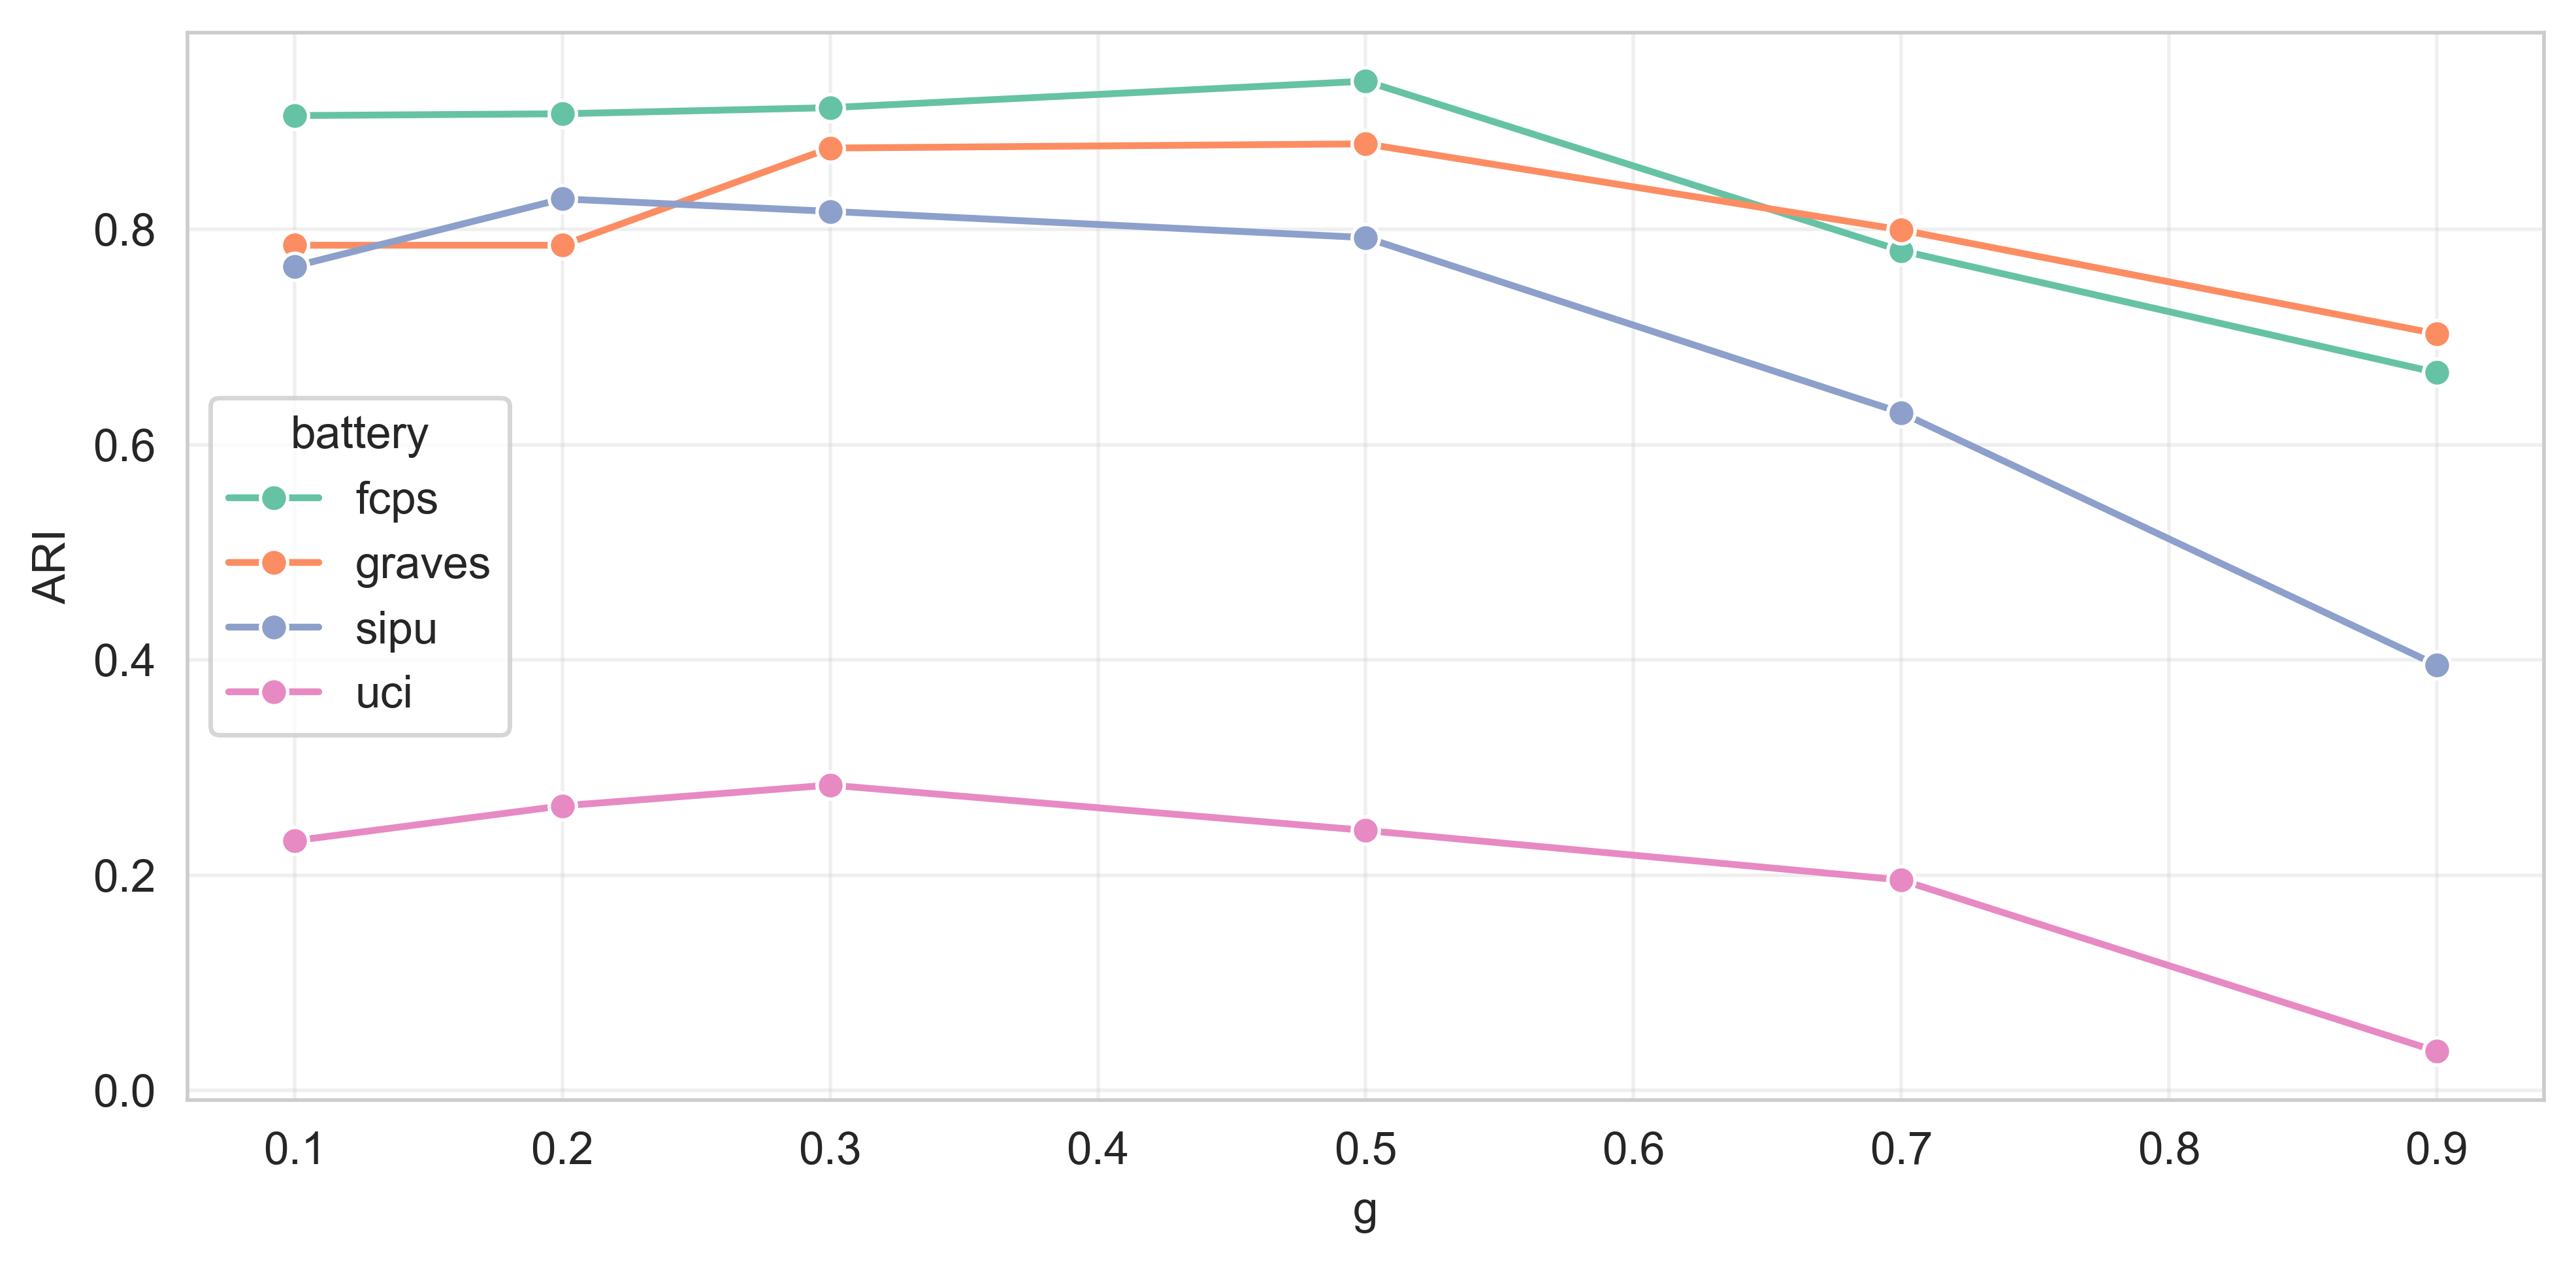
\includegraphics[width=0.88\textwidth]{genie_ari_g.png}
    \\[0.1em]
    {\small Genie is robust, but still requires moderate tuning of $g$.}
\end{frame}

\begin{frame}{ARI by Battery and Method}
    \centering
    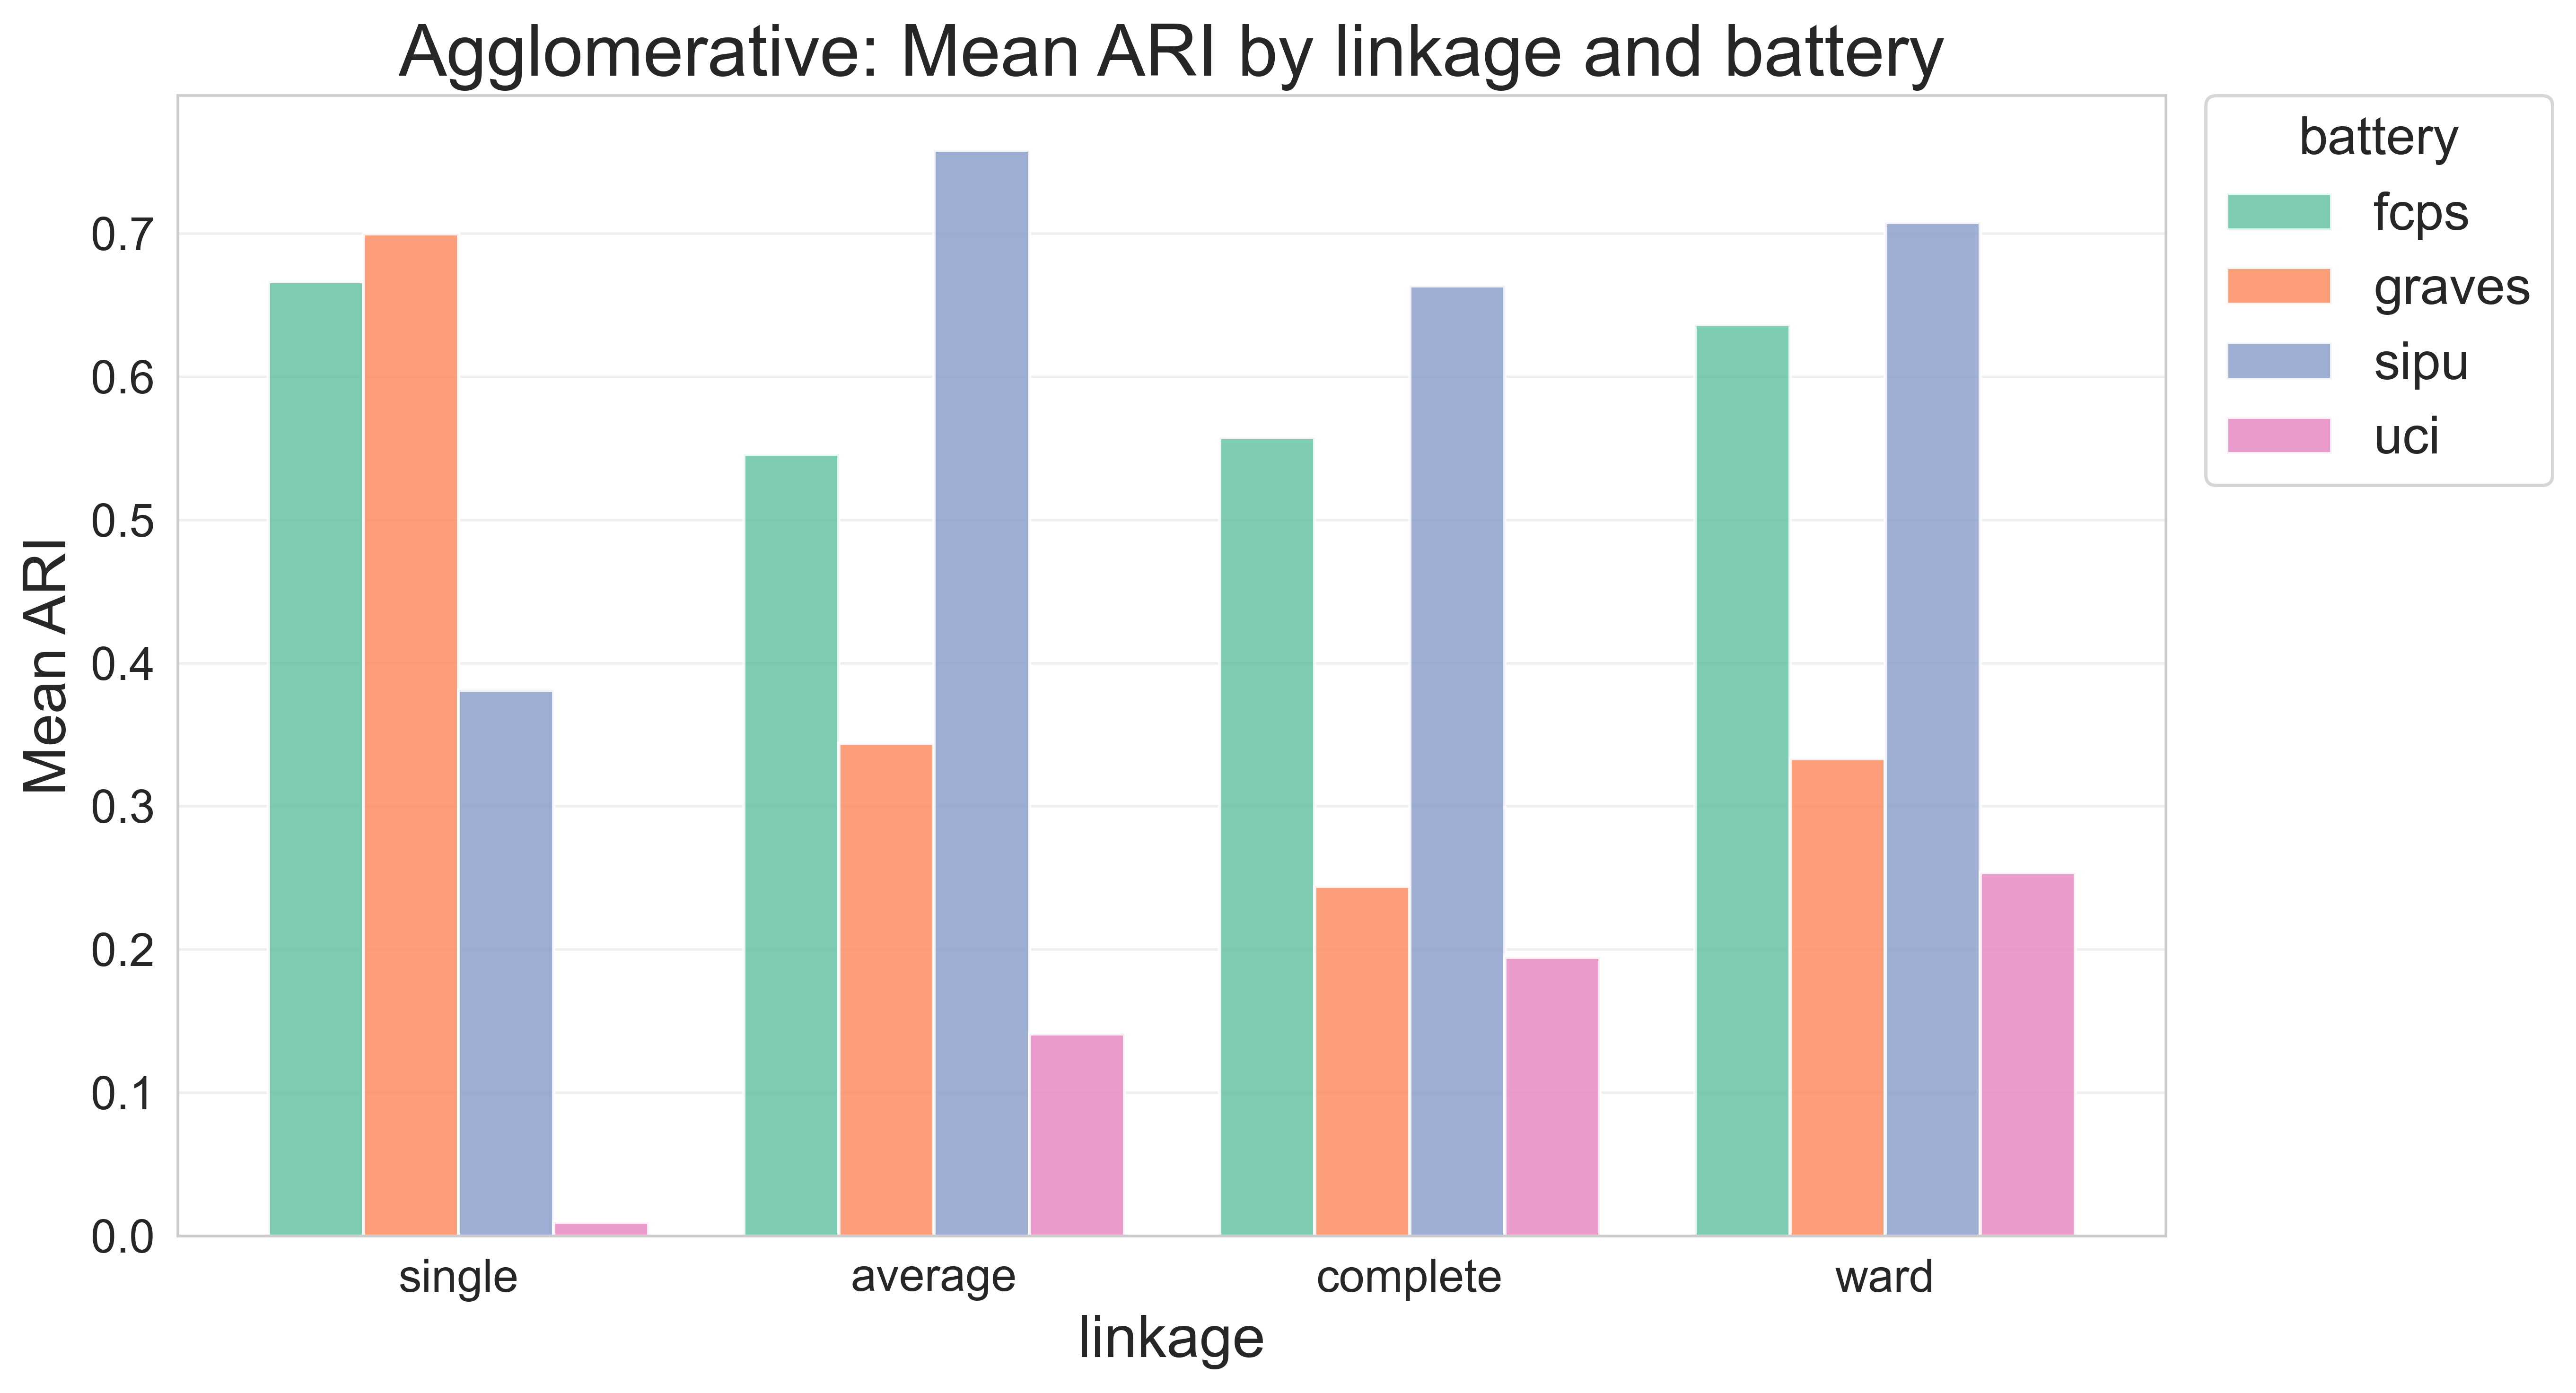
\includegraphics[width=0.92\textwidth]{agglomerative_ari_linkage.png}
    \\[0.1em]
    {\small Method effectiveness varies by battery (FCPS, Graves, SIPU, UCI).}
\end{frame}

\section{Conclusions}

\begin{frame}{Final Synthesis}
    \begin{enumerate}
        \item Genie is a strong, robust performer across datasets and metrics. Does not require extreme tuning to achieve good results.
        \item DBSCAN can achieve very high performance but is highly sensitive to hyperparameters and dataset characteristics.
        \item KMeans, Gaussian Mixture, and Spectral Clustering show stable performance.
        \item Internal metrics can be misleading if used in isolation; they should be complemented with external validation when possible. Mixed evaluation protocols are recommended for a more reliable assessment of clustering quality.
    \end{enumerate}
\end{frame}

\begin{frame}[plain]
    \centering
    \Huge \textbf{Thank You!}

    \vspace{1.5em}
    \large
    \textbf{Questions?}
\end{frame}

\end{document}
